\documentclass[11pt,a4paper]{article}
\usepackage[T1]{fontenc}
\usepackage{lmodern}
\usepackage[margin=25mm,headheight=14pt]{geometry}
\usepackage{amsmath,amssymb,amsthm,booktabs,array,graphicx}
\usepackage{xcolor,fancyhdr}
\usepackage[hidelinks]{hyperref}
\graphicspath{{../figures/}}
\pagestyle{fancy}\fancyhf{}
\fancyhead[L]{\small Geometry-attached observation retention}
\fancyhead[R]{\small Repository publication v0.1}
\fancyfoot[L]{\small Author-authorized repository research publication}
\fancyfoot[R]{\thepage}
\renewcommand{\headrulewidth}{0.3pt}
\setlength{\parindent}{0pt}\setlength{\parskip}{4pt}
\setlength{\emergencystretch}{2em}
\newcolumntype{P}[1]{>{\raggedright\arraybackslash}p{#1}}
\newtheorem{proposition}{Proposition}
\newtheorem{theorem}[proposition]{Theorem}
\newcommand{\R}{\mathbb R}\newcommand{\C}{\mathbb C}
\newcommand{\ii}{\mathrm i}\newcommand{\tr}{\operatorname{tr}}
\newcommand{\diag}{\operatorname{diag}}\newcommand{\Argz}{\operatorname{Arg}_0}
\newcommand{\ez}{e_z}\newcommand{\ee}{\mathbf1}
\newcommand{\inherited}{\textit{Inherited result.}}
\newcommand{\deduction}{\textit{SGO-01 exact specialization/deduction.}}
\newcommand{\bounded}{\textit{Bounded numerical corroboration.}}
\newcommand{\openquestion}{\textit{Open operational/physical question.}}
\title{\vspace{-12mm}\textbf{Information Retention Across\\Geometry-Attached Observations\\in the Tri-Octagon Kernel}}
\author{Hilmir Fr\'imann Halld\'orsson}
\date{7 October 2026\\\small v0.1 --- Author-authorized repository research publication}
\hypersetup{unicode=true,
pdftitle={Information Retention Across Geometry-Attached Observations in the Tri-Octagon Kernel},
pdfauthor={Hilmir Frímann Halldórsson},
pdfsubject={SGO-01 v0.1; author-authorized repository research publication; project-internal review, not external peer review},
pdfkeywords={SGO-01, geometric observation, information retention, coherence, Tri-Octagon}}
\begin{document}
\maketitle\thispagestyle{fancy}
\begin{abstract}
We determine what existing geometry-attached observations retain from a native complex triad. The complete labelled face-vector decoder is an inherited invertible representation, whereas lengths, populations, signed areas and the axial vector select different information. On the published positive SPR-01 one-update family, all signed areas and the axial vector vanish exactly, yet raw intensity is globally injective in the amplitude. A published population collision retains opposite signed coherence in the existing symmetric pair matrix. The complete mathematical axial snapshot is richer than Hermitian coherence because its quadrature accounting supplies the complex bilinear quantity $w^Tw$. We prove its static fibres: an overall-sign pair when this quantity is nonzero, an entire common-phase circle for nonzero isotropic states, and a singleton at zero. Previously executed comparisons on 205 inputs and nine static controls corroborate the unchanged implementation within a fixed numerical criterion. Exact mathematics, finite execution evidence and unresolved measurement questions remain separate. Geometry creates no new input information, and no generic inverse, full-record dynamical closure, physical realization or computational advantage is established.
\end{abstract}

\section{Question, foundations and scope}\label{sec:scope}
When a display cannot distinguish two native states, is the distinction absent from the state, lost by projection, discarded by normalization, or retained elsewhere in the existing observation record? This paper answers that question for declared observations, using one accepted input family and fixed static controls. ``Retains'' means exact mathematical identifiability unless explicitly qualified as a finite numerical comparison.

Native Response Geometry (NRG), incorporating the completed SA0 attachment analysis, supplies the decoder, representation/observation distinction and real-Gram fibre result \cite{nrg}. Paper G supplies the signed pair algebra and rank-two axial attachment \cite{paperG}. Published SPR-01 supplies the one-update family, population collision and raw/coherence inverses \cite{spr01}. SGO-01 applies these inherited results, adds the intensity and complete-record deductions below, and supplies the retained bounded comparisons \cite{sgo01}. None is a literature-wide novelty claim.

The labels \emph{inherited result}, \emph{SGO-01 exact specialization/deduction}, \emph{bounded numerical corroboration} and \emph{open operational/physical question} distinguish the sources of claims. Review and reciprocal checking were project-internal, not external peer review. This edition implies no journal acceptance, DOI, software release or physical validation.

\clearpage
\section{Adopted face representation}\label{sec:representation}
\inherited\ Write $w=x+\ii y\in\C^3$, with real channel triples $x,y$ ordered A,B,C. In the fixed canonical shell, outward unit normals and horizontal tangents are
\begin{equation}
\begin{aligned}
n_A&=(-\sqrt3/2,1/2,0),&t_A&=(-1/2,-\sqrt3/2,0),\\
n_B&=(0,-1,0),&t_B&=(1,0,0),\\
n_C&=(\sqrt3/2,1/2,0),&t_C&=(-1/2,\sqrt3/2,0),
\end{aligned}\qquad t_i=\ez\times n_i.
\label{eq:frames}
\end{equation}
The centres are $c_A=(-1/4,\sqrt3/4,0)$, $c_B=(0,0,0)$ and $c_C=(1/4,\sqrt3/4,0)$. The complete labelled representation and its encoder are
\begin{equation}
v_i=D_i(w_i)=x_it_i+y_i\ez,\qquad
E_i(v)=t_i\cdot v+\ii\ez\cdot v.\label{eq:decoder}
\end{equation}
Orthonormality of $(t_i,\ez)$ gives
\begin{equation}
E_iD_i=\mathrm{id},\qquad D_iE_i=I_3-n_in_i^T,\qquad
q_i:=\|v_i\|^2=|w_i|^2.\label{eq:inverse}
\end{equation}
Thus $ED$ is identity on $\C^3$, whereas $DE$ is only a tangent projector on ambient arrays. With labels and frames retained, the three face vectors retain all six real state coordinates, including scale and common phase \cite{nrg,kernel}.

\begin{figure}[htbp]\centering
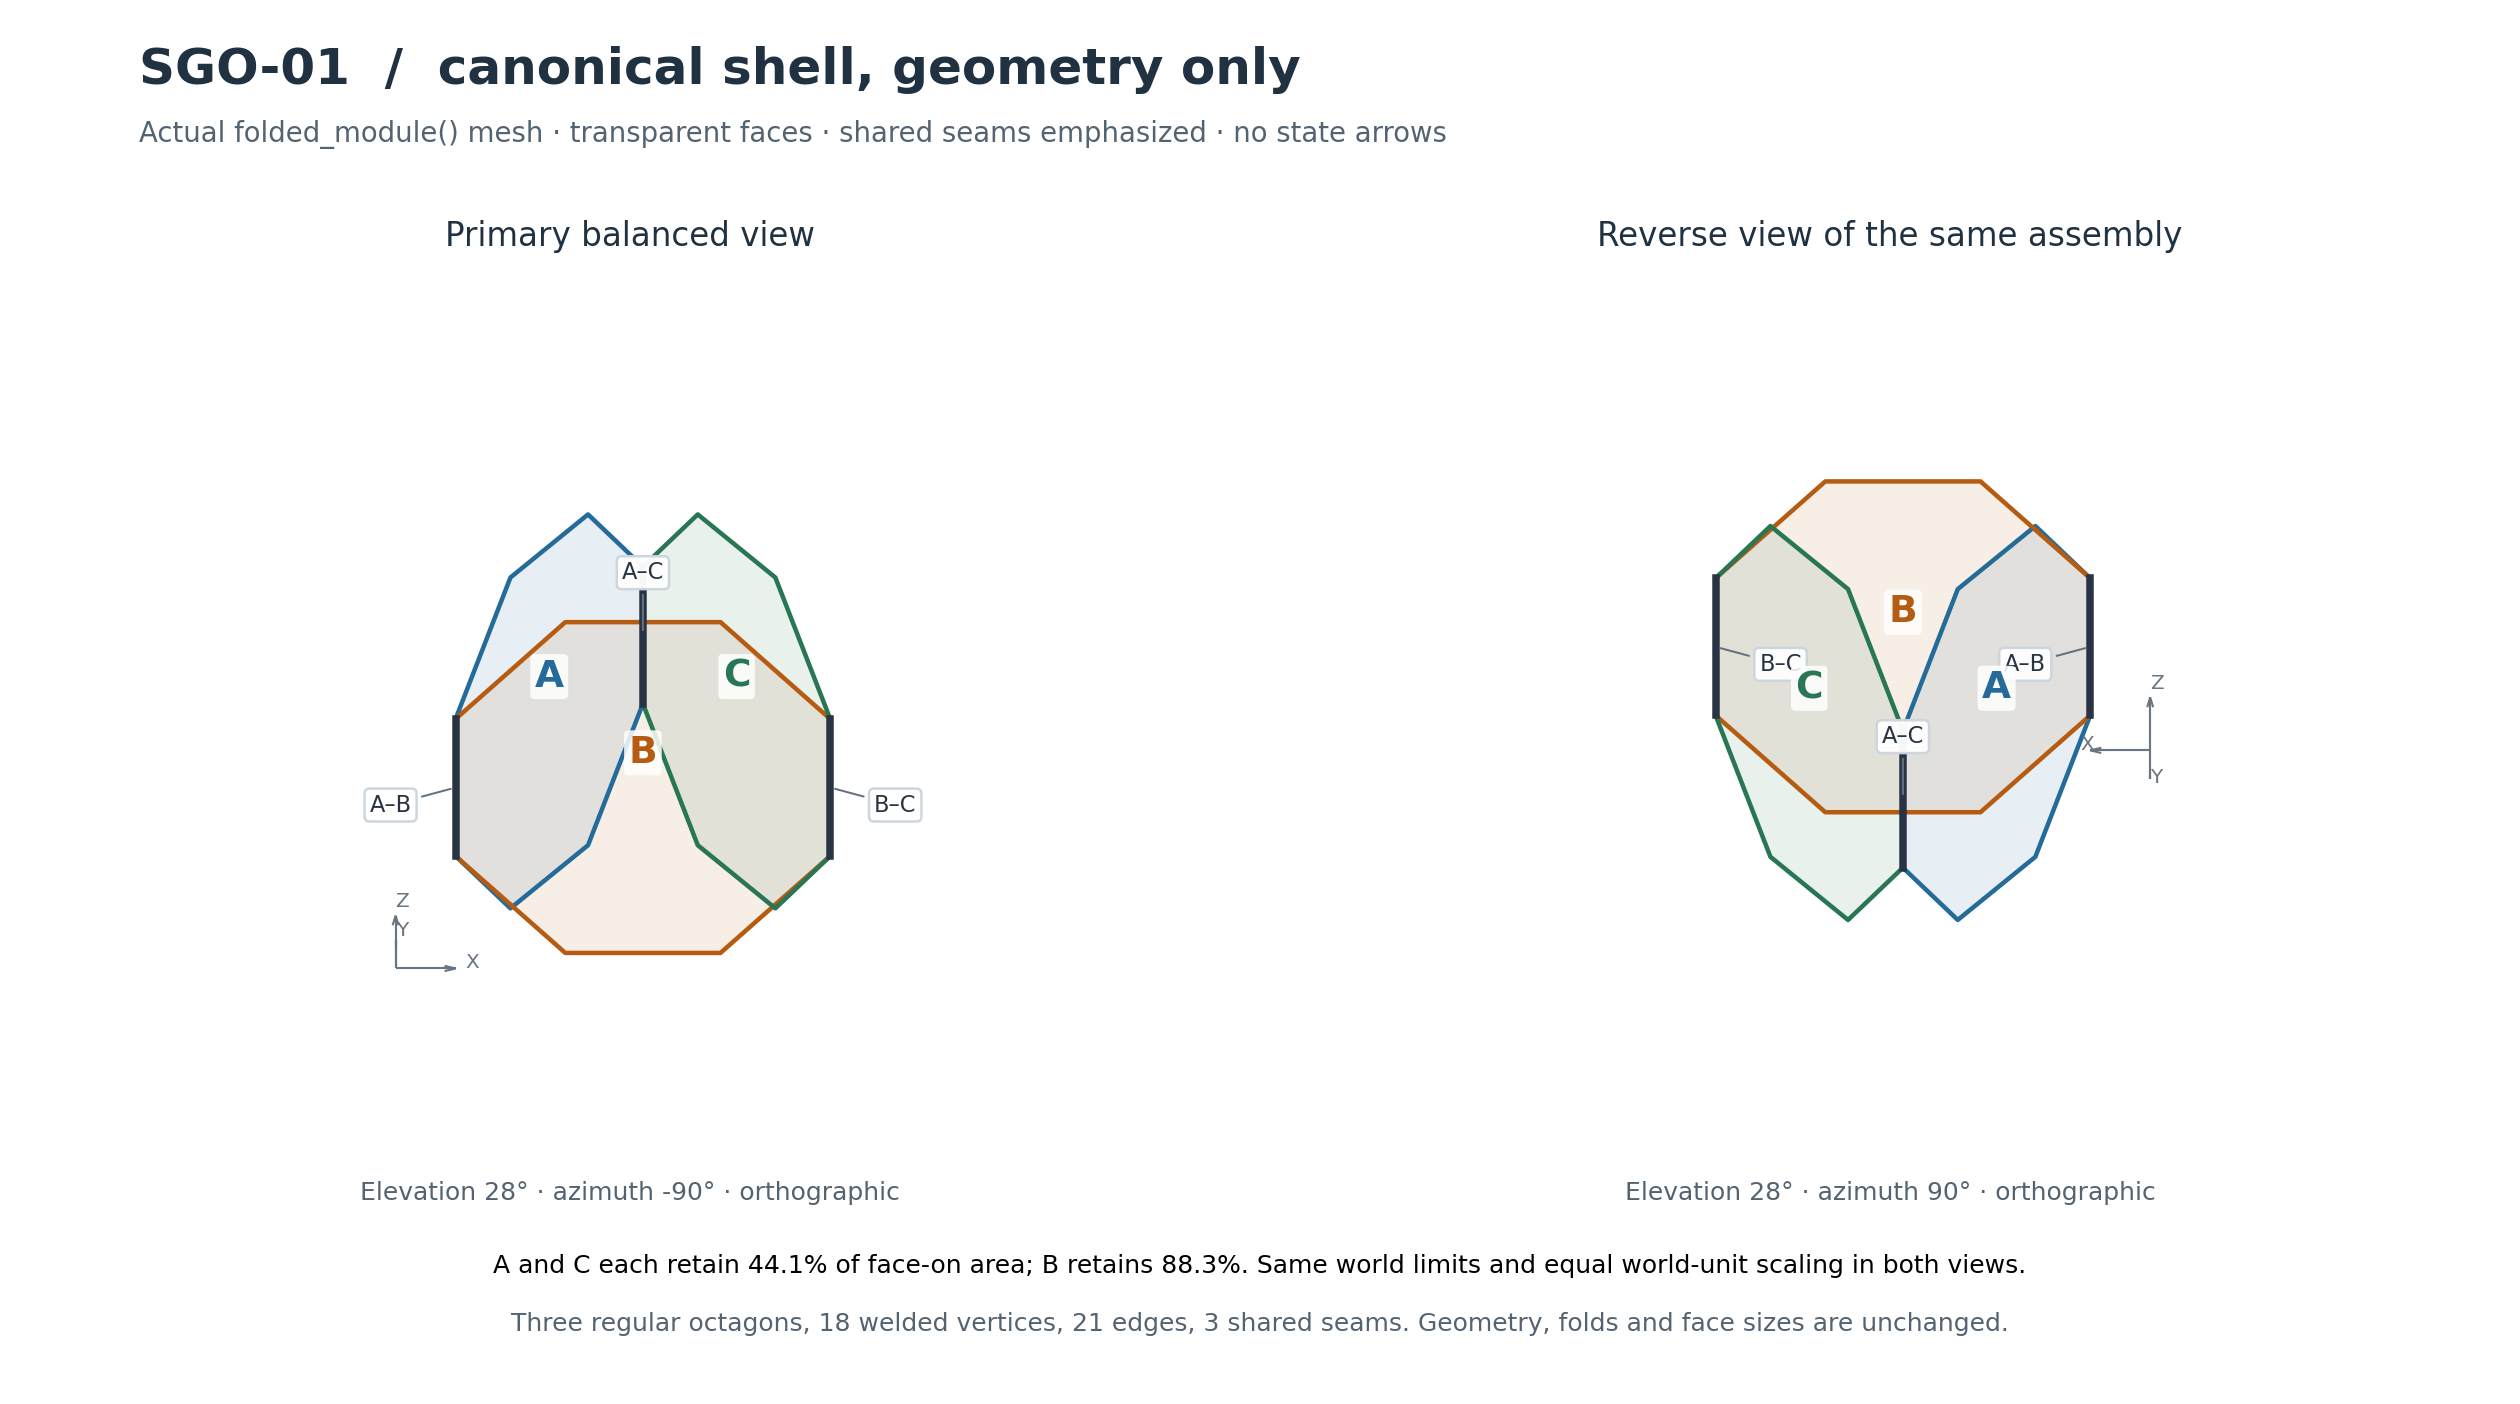
\includegraphics[width=\linewidth]{SGO01_GEOMETRY_ONLY_v02.png}
\caption{Accepted v02 geometry-only views, using the actual \texttt{geometry.folded\_module()} vertices and face cycles. A, B and C are congruent canonical regular octagons with welded, labelled shared seams. The primary and reverse cameras view the same unchanged assembly. Transparency exposes rear seams; projected face areas are not physical face sizes. There are no state arrows or deformations in this figure.}
\label{fig:geometry}
\end{figure}

The vectors in \eqref{eq:decoder} are free vectors based at fixed centres, not vertex motion, particle position, a field or a second recurrence. The internal \texttt{FaceState.step} advances stored canonical $w$ and then decodes it. It does not repeatedly evolve a rounded $E(D(w))$. Its stored state is used only for execution parity; vector reconstruction uses vectors plus frames alone.

\clearpage
\section{Matched pair data and observation hierarchy}\label{sec:hierarchy}
\inherited\ Define symmetric and antisymmetric pair matrices, Hermitian coherence and channel area by
\begin{align}
S&=xx^T+yy^T,& A&=xy^T-yx^T,& H&=ww^\dagger=S-\ii A,\label{eq:SAH}\\
C&=x\times y=(A_{BC},A_{CA},A_{AB})^T.\label{eq:C}
\end{align}
The sign in $H=S-\ii A$ distinguishes it from the conjugate coherence. Channel-area $C$ is not an ambient face vector.

\inherited\ The matched source-$j$ to destination-$i$ transport is
\begin{equation}
T_{ij}=t_it_j^T+\ez\ez^T,\qquad T_{ij}v_j=x_jt_i+y_j\ez.\label{eq:transport}
\end{equation}
Consequently the geometric pair contractions are
\begin{equation}
v_i\cdot(T_{ij}v_j)=S_{ij},\qquad
n_i\cdot\bigl(v_i\times T_{ij}v_j\bigr)=A_{ij}.\label{eq:contractions}
\end{equation}
The second identity is the inherited signed parallelogram-area convention: $t_i\times\ez=n_i$, with no factor $1/2$ \cite{paperG}. The explicit matched-dot readout is an SGO-01 specialization of the adopted transport; it is an externally calculated mathematical contraction, not a new named API or a detector.

Raw ambient dot products differ: $v_i\cdot v_j=(t_i\cdot t_j)x_ix_j+y_iy_j$. For distinct faces $t_i\cdot t_j=-1/2$. At $(21,2,21)$, for example, the untransported AB dot is $-21$, whereas $S_{AB}=42$.

\begin{table}[htbp]\centering\small
\renewcommand{\arraystretch}{1.14}
\begin{tabular}{P{.22\linewidth}P{.47\linewidth}P{.21\linewidth}}\toprule
Observation & Generic static retention/loss & Identifies positive family amplitude?\\\midrule
Labelled $D(w)$ & Entire state in the adopted frames & Yes\\
$q$; $I=\sum q_i$ & Magnitudes and scale; norm only & Yes; yes\\
$q/I$ & Normalized magnitudes, no scale or phases & No\\
$A$ or $C$ & Oriented area, not full state or intensity & No: zero\\
$W$ & Planar projection of $C$ & No: zero\\
$(W,\Gamma)$ & All of $C$, not the state & No: zero\\
$S$ & Real pair coherence, up to phase/conjugation & Yes\\
$(S,A)$ or $H$ & Nonzero state modulo common phase & Yes\\
$S/I$; $H/I$ & Also lose scale & Yes; yes\\
Complete snapshot & Equivalent to $(H,w^Tw)$; see Section~\ref{sec:snapshot} & Yes\\\bottomrule
\end{tabular}
\caption{Exact information contracts. The family column refers only to the fixed $a>0$ family in Section~\ref{sec:family}; it is not generic inversion. Named normalized bundles require $I>0$. Numerical residuals and metadata are excluded as information channels.}
\label{tab:hierarchy}
\end{table}

\clearpage
\section{Generic static losses and the axial projection}\label{sec:generic}
\subsection{Magnitudes, real Gram and complex coherence}
\inherited\ Magnitudes $q_i=|w_i|^2$ are invariant under independent channel phases; total intensity retains only the norm. Division by $I$ also loses positive scale. These statements do not imply that the same losses persist on every restricted family.

The generic real-Gram fibre characterization is inherited from NRG's regular real-Gram closure proof, including its rank-deficient factor argument \cite{nrg}. For completeness, write $B=[x\ y]$, so $S=BB^T$. Equal row Gram matrices determine an isometry of the spanned row spaces, extending to an $O(2)$ transformation: $B'=BO$. Rotations give common phase, and reflections give common phase followed by conjugation. Hence
\begin{equation}
S(w')=S(w)\quad\Longleftrightarrow\quad
w'=e^{\ii\theta}w\ \text{or}\ w'=e^{\ii\theta}\overline w.
\label{eq:Sfibre}
\end{equation}
This inherited result is applied here, not claimed as a new SGO-01 theorem. For nonzero $H=ww^\dagger$, equality fixes the same rank-one complex range, so $w'=cw$ with $|c|=1$. Thus $H$ retains the state modulo common phase; $H/I$ retains only its complex line, with arbitrary $c\ne0$. Normalized $S/I$ adds positive-scale ambiguity to \eqref{eq:Sfibre}. Zero has a singleton unnormalized $S$ or $H$ fibre.

These are static information statements. NRG's regular closure results require nonzero pre-synchronization components; the native zero convention supplies a separate obstruction. A static fibre description alone is not a full-domain autonomous update law.

\subsection{What the axial vector discards}
\inherited\ Let $e=(1,1,1)^T$. Paper G's ambient attachment uses
\begin{equation}
T=\begin{pmatrix}-1/2&1&-1/2\\-\sqrt3/2&0&\sqrt3/2\\0&0&0\end{pmatrix},
\qquad W=TC,\qquad\Gamma=e^TC.\label{eq:attachment}
\end{equation}
This $T$, with columns $t_i$, differs from $T_{ij}$. Its column inner products give
\begin{equation}
T^TT=\frac32\left(I_3-\frac{ee^T}{3}\right),\qquad
\ker T=\R e,\qquad C=\frac23T^TW+\frac\Gamma3e.\label{eq:recoveryC}
\end{equation}
Thus $(W,\Gamma)$ recovers $C$, whereas $W=0$ only implies $C\parallel e$. Neither observation generally determines the state or its intensity. For example, $x\mapsto tx$, $y\mapsto y/t$ preserves $C$ for nonzero real $t$ while generally changing intensity. Also $C=0$ exactly when $x,y$ are collinear, including every real state.

\deduction\ The prescribed static control $v=(1,-1+\ii,-\ii)$ has $x=(1,-1,0)$, $y=(0,1,-1)$, hence $C=(1,1,1)$, $W=0$ and $\Gamma=3$. It exhibits area hidden by the projection, not an evolved trajectory or a physical field effect. This applies the inherited reconstruction theorem rather than replacing it.

\clearpage
\section{The fixed SPR-01 one-update family}\label{sec:family}
\inherited\ The native triad update first forms an amplitude prestage and then synchronizes phases simultaneously:
\begin{align}
u&=z+\epsilon z\odot(k-|z|^2)+gLz,&L&=ee^T-3I_3,\label{eq:prestage}\\
F_i(z)&=|u_i|e^{\ii(\phi_i+\delta_i)},&
\delta_i&=\lambda\sum_{j\ne i}\sin\bigl(3(\phi_j-\phi_i)\bigr),\label{eq:F}
\end{align}
where $\phi_i=\Argz(u_i)$, $\Argz(0)=0$, and zero prestage components produce zero outputs \cite{paperA,kernel}. There is no normalization or geometric feedback in this recurrence.

The accepted SPR-01 settings are
\begin{equation}
z(a)=a(1,2,1)^T,\quad a>0,\quad
\epsilon=\frac1{20},\quad g=\frac15,\quad\lambda=\frac1{30},\quad k=(1,1,1).
\label{eq:settings}
\end{equation}
One update is applied to each independently prepared input. Substitution into \eqref{eq:prestage} gives the inherited exact response
\begin{equation}
w(a)=F(z(a))=\frac a{20}(25-a^2,34-8a^2,25-a^2)^T.\label{eq:w}
\end{equation}
All nonzero prestage phases are $0$ or $\pi$, so the threefold sine increments vanish exactly. The zero convention leaves any cancelled component zero. Thus \eqref{eq:w} is the full update, not only the prestage \cite{spr01}.

\deduction\ Set $X=a^2$, $s=25-X$, $r=17-4X$ and $d=s^2+2r^2$. The existing face and pair observations specialize to
\begin{equation}
D(w)=\begin{pmatrix}-as/40&-\sqrt3as/40&0\\ar/10&0&0\\-as/40&\sqrt3as/40&0\end{pmatrix},
\quad q=\frac{a^2}{400}(s^2,4r^2,s^2)^T,\label{eq:familyDq}
\end{equation}
\begin{equation}
S=H=\frac{a^2}{400}
\begin{pmatrix}s^2&2sr&s^2\\2sr&4r^2&2sr\\s^2&2sr&s^2\end{pmatrix},
\qquad A=C=W=\Gamma=0.\label{eq:familyS}
\end{equation}
The two factors $s,r$ cannot vanish together, so $I=a^2d/200>0$ for every $a>0$. Dividing \eqref{eq:familyDq} and \eqref{eq:familyS} by $I$ gives $q/I=(s^2,4r^2,s^2)^T/(2d)$ and the displayed matrix divided by $2d$. Also $A/I=0$. A zero axial arrow is therefore entirely uninformative about amplitude on this family, while the complete vectors remain nonzero. Quadrature accounting has $Q_x=I$, $Q_y=h=0$; its meaning is developed in Section~\ref{sec:snapshot}.

\clearpage
\section{Intensity injectivity and inverse domains}\label{sec:intensity}
\begin{theorem}[SGO-01 exact deduction: positive-family intensity]
The inherited output-intensity polynomial
\begin{equation}
I(a)=\frac{a^2(33a^4-322a^2+1203)}{200}\label{eq:intensity}
\end{equation}
is a bijection from $a>0$ to $I>0$.
\end{theorem}
\begin{proof}
Differentiation and completing the square give
\begin{equation}
I'(a)=\frac a{100}\left[99\left(a^2-\frac{322}{99}\right)^2+\frac{15413}{99}\right]>0.\label{eq:derivative}
\end{equation}
Also $I(a)\to0$ as $a\to0^+$ and $I(a)\to\infty$ as $a\to\infty$. Continuity and strict monotonicity prove the claim.
\end{proof}
Given $I>0$, there is a unique positive solution $X$ of
\begin{equation}
33X^3-322X^2+1203X=200I,\qquad a=\sqrt X.\label{eq:cubicinverse}
\end{equation}
Consequently raw $q$, $S$ and the full snapshot also identify $a$. This is exact identifiability on a known family, not generic sign detection, an inverse-conditioning estimate or a finite-noise theorem. Generic states $(21,2,21)$ and $(21,-2,21)$ have equal intensity but different relative sign. Entrance intensity $6a^2$ already identifies positive $a$; geometry does not create that information.

\inherited\ The SPR-01 raw inverse and normalized-coherence chart are
\begin{equation}
a=\frac{10}{83}(8w_A-w_B),\qquad
t=\frac{(S/I)_{BA}}{2(S/I)_{AA}}=\frac{17-4X}{25-X},\qquad
a=\sqrt{\frac{17-25t}{4-t}}.\label{eq:inverses}
\end{equation}
The chart requires $a\ne5$. Its projective injectivity follows from
\begin{equation}
(25-X)(17-4Y)-(17-4X)(25-Y)=83(X-Y).\label{eq:projective}
\end{equation}
At $a=5$, the unique pure-B normalized direction identifies the exceptional point. Since $S=H$ on this real family, $S/I$ alone suffices \cite{spr01}.

\begin{table}[htbp]\centering\small
\begin{tabular}{P{.16\linewidth}P{.41\linewidth}P{.33\linewidth}}\toprule
Input & Exact output and intensity & Normalized status\\\midrule
$a=0$ & $w=0$, $I=0$ & Undefined; outside $a>0$\\
$a=\sqrt{17}/2$ & $w=(83\sqrt{17}/160,0,83\sqrt{17}/160)$; $I=117113/12800$ & $q/I=(1/2,0,1/2)$; $S/I=\tfrac12\left(\begin{smallmatrix}1&0&1\\0&0&0\\1&0&1\end{smallmatrix}\right)$\\
$a=5$ & $w=(0,-83/2,0)$; $I=6889/4$ & $q/I=(0,1,0)$; $S/I=\diag(0,1,0)$\\\bottomrule
\end{tabular}
\caption{Zero and component cancellations. $A/I=0$ at both nonzero cancellations. These exact family values do not extend the earlier general nonzero-prestage closure theorem through its excluded points.}
\label{tab:domains}
\end{table}

\clearpage
\section{Same populations, different retained information}\label{sec:pair}
\inherited\ SPR-01's collision uses two unequal-scale outputs, at
\begin{equation}
a=2,\qquad b=\sqrt{382/85},\qquad \kappa=\frac{83b}{1700},\qquad
w(2)=\frac1{10}(21,2,21),\quad w(b)=\kappa(21,-2,21).\label{eq:pair}
\end{equation}
Let
\begin{equation}
M_\pm=\begin{pmatrix}441&\pm42&441\\\pm42&4&\pm42\\441&\pm42&441\end{pmatrix}.
\label{eq:Mpm}
\end{equation}
\deduction\ The complete raw/readout comparison specializes the inherited collision as follows:
\begin{table}[htbp]\centering
\renewcommand{\arraystretch}{1.3}
\begin{tabular}{lll}\toprule
Readout & $a=2$ & $a=b$\\\midrule
$q$ & $(441,4,441)/100$ & $\kappa^2(441,4,441)$\\
$I$ & $443/50=8.86$ & $582898957/61412500$\\
$S=H$ & $M_+/100$ & $\kappa^2M_-$\\
$q/I$ & $(441,4,441)/886$ & $(441,4,441)/886$\\
$S/I=H/I$ & $M_+/886$ & $M_-/886$\\
$(S/I)_{AB}$ & $+21/443$ & $-21/443$\\
$A,C,W,\Gamma$ & All zero & All zero\\
$(Q_x,Q_y,h)$ & $(443/50,0,0)$ & $(582898957/61412500,0,0)$\\\bottomrule
\end{tabular}
\caption{Actual ideal outputs of the two published amplitudes, not the equal-scale sign controls. The vectors are $D(w(2))$ and $D(w(b))$ under the same fixed decoder.}
\label{tab:pair}
\end{table}

The second intensity is approximately $9.49153603908$, and
\begin{equation}
I(b)-I(2)=\frac{38784207}{61412500}>0.\label{eq:intensitygap}
\end{equation}
Thus identical normalized populations do not imply equal raw lengths or intensity. The opposite signed coherence survives in the already-existing $S$ field, in $H$, in their normalized versions, in the full snapshot and in matched geometric dot products. It is not stored in $A$, which vanishes for both ideal real outputs.

The fixed equal-scale controls $r_+=(21,2,21)$ and $r_-=(21,-2,21)$ isolate a different point: both have $q=(441,4,441)$ and $I=886$, but $S=M_+$ versus $M_-$. This demonstrates loss of relative sign by magnitude-only observation without attributing generic sign detection to raw intensity. Figure~\ref{fig:comparison} uses the actual unequal-scale native outputs, preserving their saved floating-point components.

\clearpage
\begin{figure}[p]\centering
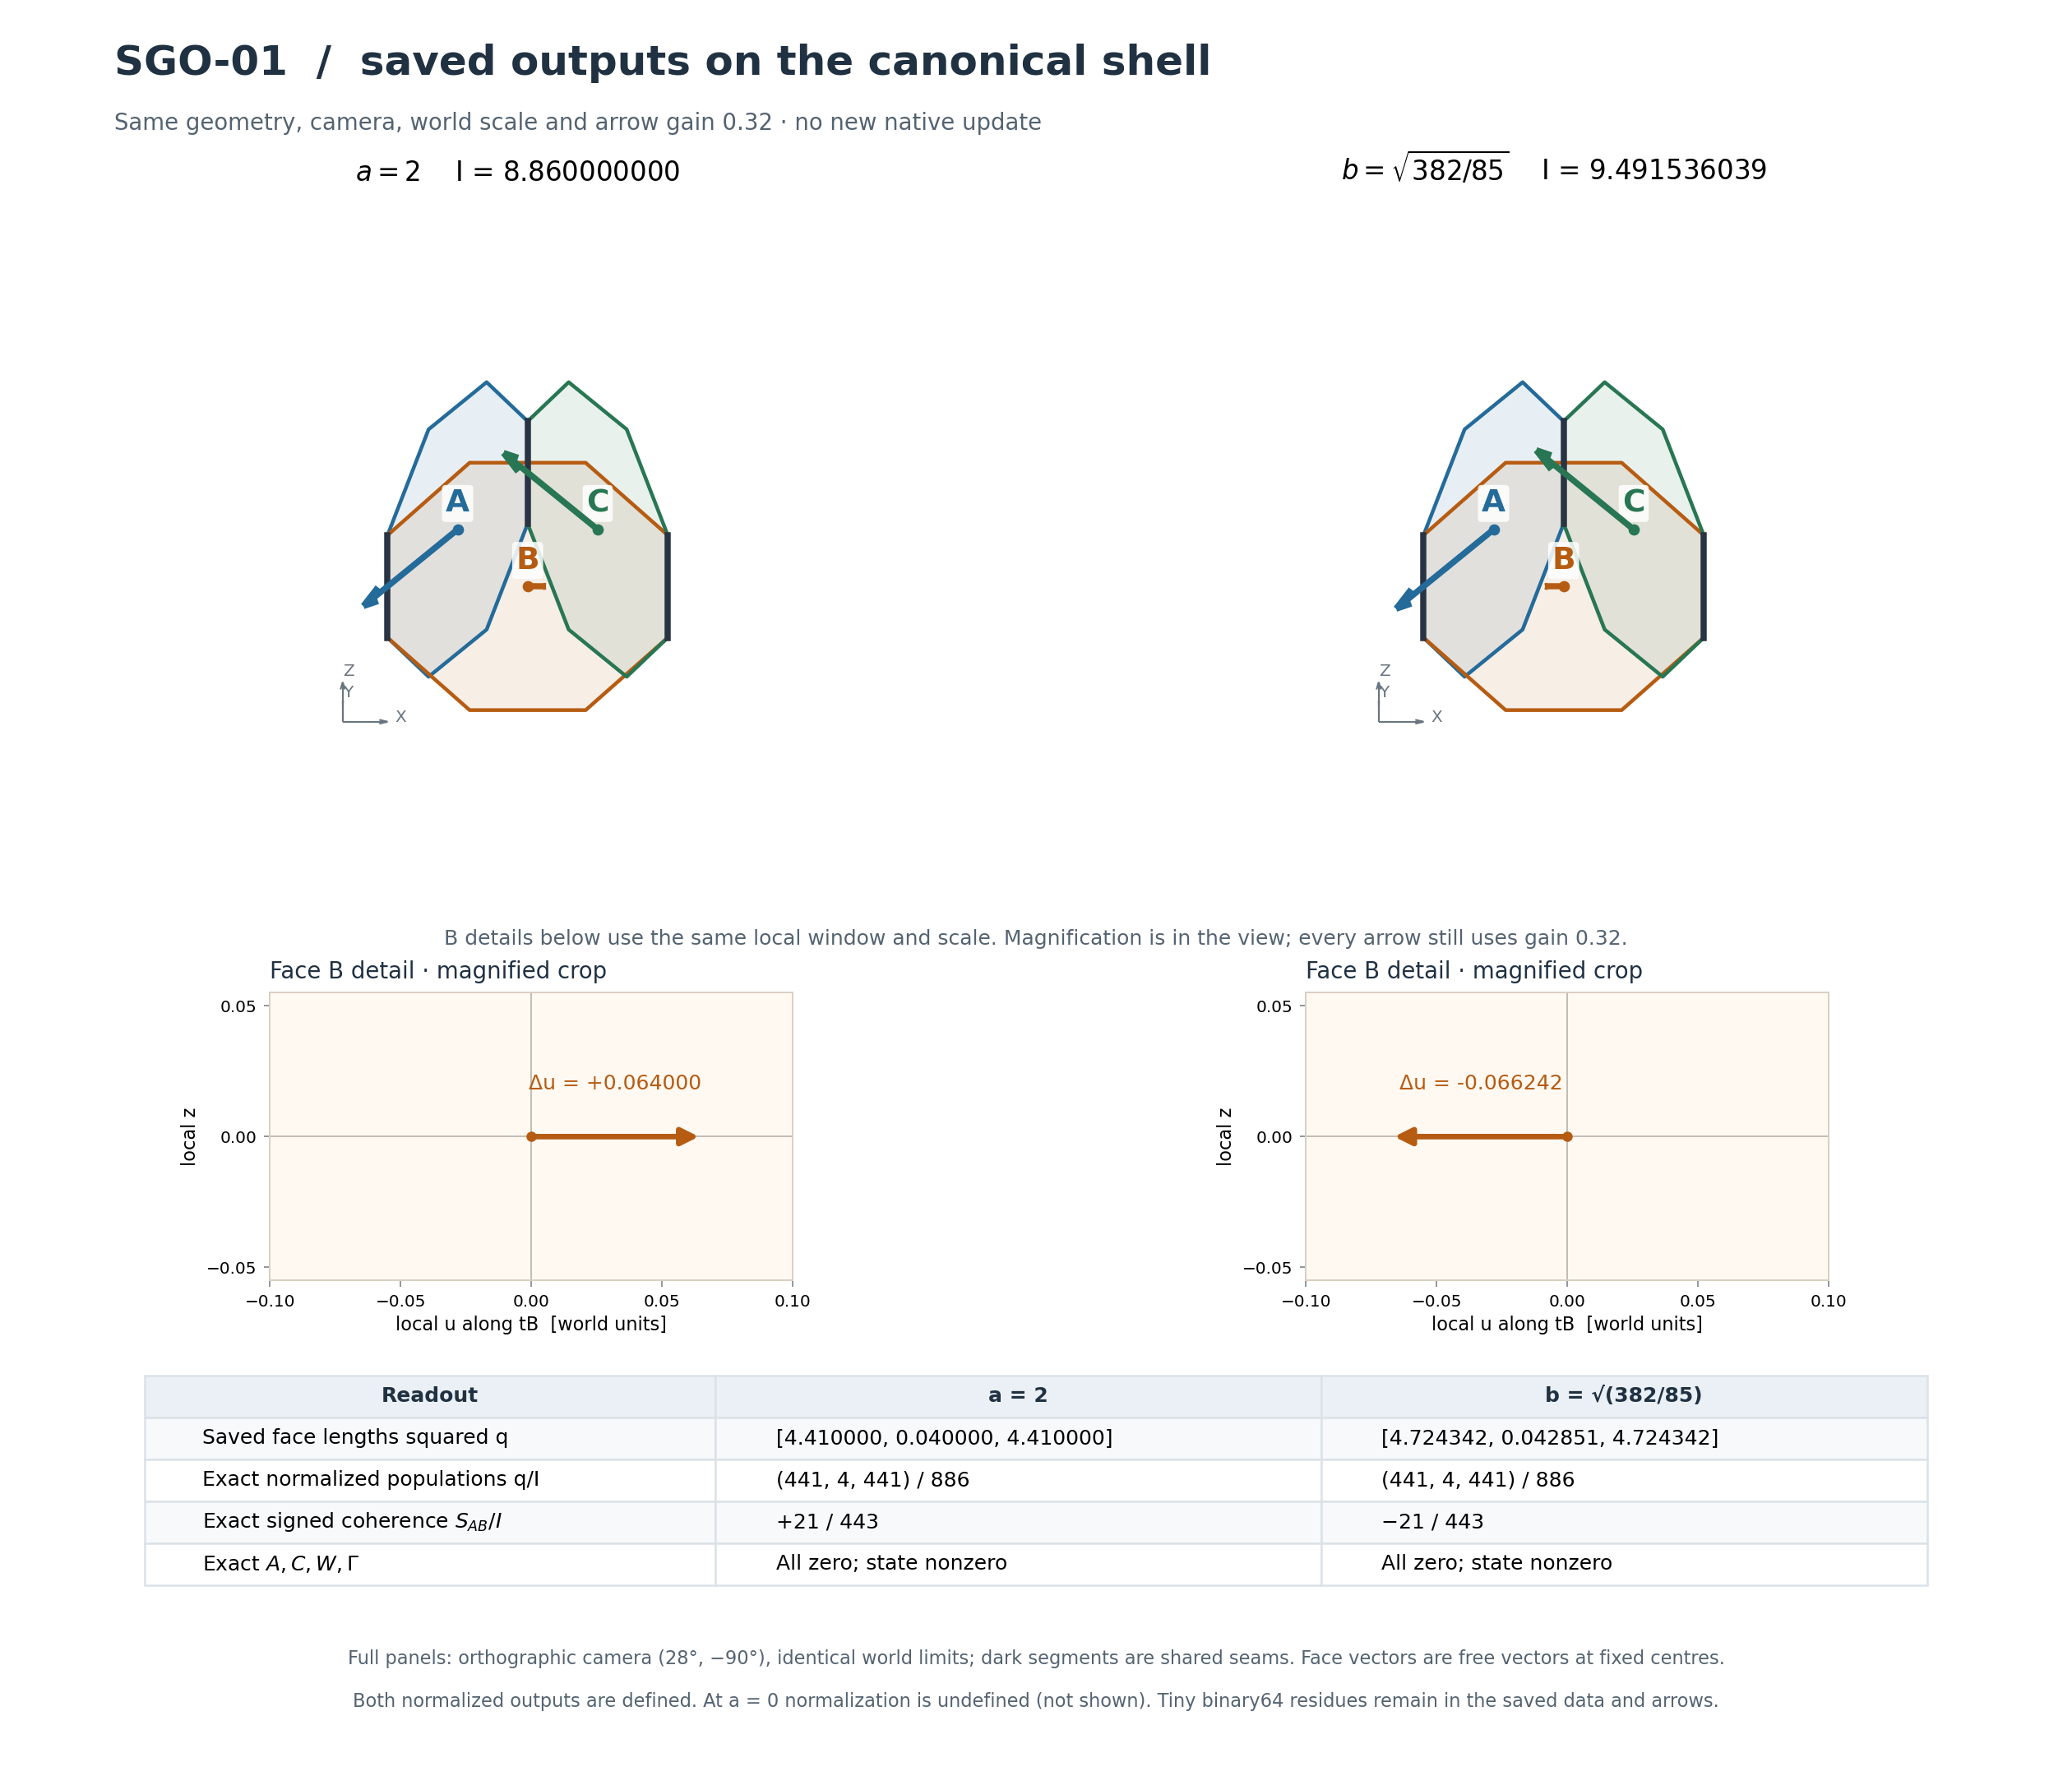
\includegraphics[width=\linewidth]{SGO01_FACE_READOUT_COMPARISON_v02.png}
\caption{Accepted v02 comparison of two separately prepared one-update outputs, not successive frames. The top panels use the same canonical regular-octagon assembly, welded shared seams, orthographic camera, world scaling and arrow gain $0.32$. Arrows are free state vectors at fixed face centres, not deformation, force, field lines or particle displacement. The labelled B-detail panels are magnified local crops with identical limits and unchanged arrow gain, making the sign reversal readable. Saved binary64 residues are retained; exact zero-area labels describe the ideal real family. The full-resolution PNG accompanies this edition.}
\label{fig:comparison}
\end{figure}
\clearpage

\section{Complete snapshot information and phase qualification}\label{sec:snapshot}
\inherited\ The existing public \texttt{AxialSnapshot} includes $S,A,C,W,\Gamma,I$, area decomposition and norms, quadrature accounting, residuals and constant metadata \cite{kernel}. It is not merely $W$, and it is not a squared-magnitude-only record. In particular,
\begin{equation}
Q_x=\|x\|^2,\qquad Q_y=\|y\|^2,\qquad h=x\cdot y,\qquad I=Q_x+Q_y.\label{eq:quadrature}
\end{equation}
These are the accounting fields named \texttt{A}, \texttt{B} and \texttt{h}; the first is not the antisymmetric matrix $A$.

\begin{table}[htbp]\centering\small
\renewcommand{\arraystretch}{1.15}
\begin{tabular}{P{.38\linewidth}P{.54\linewidth}}\toprule
Field group & Exact information content\\\midrule
$S,A$ & $H=S-\ii A$\\
$C,\Gamma,C_\parallel,C_\perp,W$ & $C$ from $A$; $\Gamma=e^TC$; $C_\parallel=\Gamma e/3$; $C_\perp=C-C_\parallel$; $W=TC$\\
Intensity and area/axial norms & $I=\tr S$, $\|C\|$, $\|W\|$\\
Accounting $Q_x,Q_y,h$ & Additional quadrature-reference information\\
Accounting Gram and slack fields & $Q_xQ_y$, $h^2$, $Q_xQ_y-h^2=\|C\|^2$; $I/2$; $(Q_x-Q_y)^2/4+h^2=I^2/4-\|C\|^2$\\
Duplicate accounting fields & $C,I,\|C\|,\|C\|^2$\\
Residuals & Zero in exact mathematics; finite-arithmetic diagnostics\\
Revision/source/policy metadata & Constants, not state information\\\bottomrule
\end{tabular}
\caption{The entire mathematical record reduces to $H$ and $(Q_x,Q_y,h)$. Heterogeneous metadata and numerical residuals are not normalized or treated as hidden recovery channels.}
\label{tab:snapshot}
\end{table}
The residuals express $A+[C]_\times=0$, $SC=0$, \eqref{eq:recoveryC}, $W_z=0$, and
\begin{equation}
e_2(S)=\|C\|^2,\qquad I^2-|w^Tw|^2=4\|C\|^2,\qquad
\|C\|^2=\frac{2\|W\|^2+\Gamma^2}{3},\label{eq:residuals}
\end{equation}
as well as the Gram/slack equalities in Table~\ref{tab:snapshot}. Here $[C]_\times v=C\times v$ and $e_2$ sums principal $2\times2$ minors.

\deduction\ The older shorthand ``snapshot common-phase invariance'' must be restricted to the selected invariant fields $S,A,C,W,\Gamma,I$ \cite{axialcontract}. It does not describe the entire heterogeneous record: at $r_+$ the accounting pair is $(Q_x,Q_y)=(886,0)$, whereas at $\ii r_+$ it is $(0,886)$, despite identical $H$. This is a documentation-scope qualification; no runtime field is removed or changed. NRG's regular $H/S$ closure result cannot automatically be promoted to full-record closure.

\clearpage
\subsection{Static fibres of the complete mathematical record}
\begin{theorem}[SGO-01 exact deduction: complete-record fibres]\label{thm:snapshot}
Excluding constant metadata and floating residuals, the snapshot retains exactly the information in $(H,\beta)$, where
\begin{equation}
\beta(w)=w^Tw=Q_x-Q_y+2\ii h.\label{eq:beta}
\end{equation}
Its fibre at $w$ is $\{w,-w\}$ if $\beta(w)\ne0$; it is $\{e^{\ii\theta}w:\theta\in\R\}$ if $w\ne0$ and $\beta(w)=0$; and it is $\{0\}$ at zero.
\end{theorem}
\begin{proof}
Table~\ref{tab:snapshot} shows that the whole record is a function of $H,Q_x,Q_y,h$, which conversely occur among its fields. Since $H$ supplies $I=Q_x+Q_y$, \eqref{eq:beta} recovers $Q_x=(I+\Re\beta)/2$, $Q_y=(I-\Re\beta)/2$, $h=\Im\beta/2$.

For $w\ne0$, any state with equal $H$ has form $w'=e^{\ii\theta}w$. But $\beta(w')=e^{2\ii\theta}\beta(w)$. If $\beta\ne0$, equality requires $e^{2\ii\theta}=1$, giving exactly $w$ and $-w$. If $\beta=0$, then $Q_x=Q_y=I/2$ and $h=0$, unchanged by every common phase. Finally $H=0$ forces $w=0$.
\end{proof}
The additional phase reference is a reference in the supplied complex coordinates, not a physical apparatus. These fibres are static; the theorem is neither an inverse of $F$ nor a complete-snapshot dynamical closure law.

\subsection{The nine fixed static controls}\label{sec:controls}
\deduction\ Let $q_r=(441,4,441)$ and use $M_\pm$ from \eqref{eq:Mpm}. All prescribed controls in Table~\ref{tab:controls} are unevolved observer inputs. Their exact normalized bundles follow by dividing $q,S,A$ individually by the nonzero $I$.
\begin{table}[htbp]\centering\small
\renewcommand{\arraystretch}{1.1}
\begin{tabular}{lllll}\toprule
State & $q$; $I$ & $S$; $A$ & $C$; $\Gamma$ & $(Q_x,Q_y,h)$\\\midrule
$r_+$ & $q_r$; $886$ & $M_+$; $0$ & $0$; $0$ & $(886,0,0)$\\
$r_-$ & $q_r$; $886$ & $M_-$; $0$ & $0$; $0$ & $(886,0,0)$\\
$-r_+$ & $q_r$; $886$ & $M_+$; $0$ & $0$; $0$ & $(886,0,0)$\\
$\ii r_+$ & $q_r$; $886$ & $M_+$; $0$ & $0$; $0$ & $(0,886,0)$\\
$2r_+$ & $4q_r$; $3544$ & $4M_+$; $0$ & $0$; $0$ & $(3544,0,0)$\\
$u=(1,\ii,0)$ & $(1,1,0)$; $2$ & $S_u$; $A_u$ & $(0,0,1)$; $1$ & $(1,1,0)$\\
$\overline u$ & $(1,1,0)$; $2$ & $S_u$; $-A_u$ & $(0,0,-1)$; $-1$ & $(1,1,0)$\\
$\ii u$ & $(1,1,0)$; $2$ & $S_u$; $A_u$ & $(0,0,1)$; $1$ & $(1,1,0)$\\
$v=(1,-1+\ii,-\ii)$ & $(1,2,1)$; $4$ & $S_v$; $A_v$ & $(1,1,1)$; $3$ & $(2,2,-1)$\\\bottomrule
\end{tabular}
\caption{Exact static controls. $W=TC$ throughout. The complex controls isolate conjugation, an isotropic common-phase ambiguity and area hidden by the planar projection.}
\label{tab:controls}
\end{table}

\clearpage
\subsection{Explicit control matrices and interpretation}
The matrices used in Table~\ref{tab:controls} are
\begin{equation}
S_u=\diag(1,1,0),\quad
A_u=\begin{pmatrix}0&1&0\\-1&0&0\\0&0&0\end{pmatrix},\quad
W(u)=(-1/2,\sqrt3/2,0),\label{eq:u}
\end{equation}
\begin{equation}
S_v=\begin{pmatrix}1&-1&0\\-1&2&-1\\0&-1&1\end{pmatrix},\qquad
A_v=\begin{pmatrix}0&1&-1\\-1&0&1\\1&-1&0\end{pmatrix}.\label{eq:v}
\end{equation}
The controls separate loss of relative sign ($r_+,r_-$), global sign ($r_+,-r_+$), quadrature-reference phase ($r_+,\ii r_+$), scale under normalization ($r_+,2r_+$), and area orientation ($u,\overline u$). Since $u^Tu=0$, $u$ and $\ii u$ have the same entire mathematical snapshot, even though their complete face vectors differ. For $v$, nonzero $C$ is hidden in $W$ but recovered by $\Gamma$. These are applications of the explicit formulas and Theorem~\ref{thm:snapshot}; no additional evolved controls were introduced.

\section{Bounded implementation evidence}\label{sec:evidence}
\bounded\ The completed study froze the following comparison before execution \cite{sgo01}:
\begin{equation}
a_j=\frac12+\frac j{100},\quad j=0,\ldots,200,
\quad\text{plus }\sqrt{17}/2,\ \sqrt{382/85},\label{eq:grid}
\end{equation}
giving 203 main-window inputs. The separately flagged diagnostics $a=0,5$ give 205 distinct inputs. Each was evaluated once through each of three existing paths: native \texttt{step3} followed by face/axial observation; internal \texttt{FaceState.step(config, profile=None)}; and public \texttt{api.step(State(...), Parameters(...), topology="triad")} followed by \texttt{api.axial\_snapshot}. This yields 615 update-route evaluations, not 615 distinct inputs. Nine static controls through native/public observers add 18 records without updates.

An independent exact/100-digit reference used explicit radical frames rather than the rounded frames being tested. Three error levels were separated: state error against ideal $w(a)$; observer error against formulas on the exact supplied binary64 components; and end-to-end readout error against ideal $w(a)$. Binary64 components were lifted by integer ratios. Each named field used the frozen criterion
\begin{equation}
\mathrm{error}\le10^{-12}+10^{-10}\|\mathrm{reference}\|,\label{eq:criterion}
\end{equation}
with absolute scalar, Euclidean vector and Frobenius matrix norms. Undefined normalized fields at zero were null, not zero. No phase alignment, clipping, forced zeros, sign repair or tolerance retuning occurred. This criterion is numerical, not a physical measurement-noise assumption.

All 205 route triples had byte-identical canonical states and equal named observations; all nine static native/public pairs agreed. The 204 inputs shared with original SPR-01 reproduced its saved native/public output bytes. No checked-arithmetic refusal occurred. These are finite execution findings, not uniform guarantees outside the fixtures or installed-UI certification.

\clearpage
\subsection{Recorded errors, independent audit and passivity}
\bounded\ Across the 203 main-window inputs, the maximum raw native-state error was $1.7281369134961648\times10^{-15}$. Representative field maxima are shown in Table~\ref{tab:errors}; the other routes agree.
\begin{table}[htbp]\centering\small
\renewcommand{\arraystretch}{1.15}
\begin{tabular}{lrr}\toprule
Field & Observer-only error & End-to-end error\\\midrule
Complete face vectors & $4.5221\times10^{-16}$ & $1.7257\times10^{-15}$\\
$q$ vector & $2.4522\times10^{-15}$ & $6.5431\times10^{-15}$\\
Snapshot intensity & $1.5550\times10^{-15}$ & $9.2304\times10^{-15}$\\
$S$ & $8.8730\times10^{-16}$ & $1.0751\times10^{-14}$\\
$A$ & $1.3555\times10^{-31}$ & $1.2629\times10^{-15}$\\
$C$ & $9.5847\times10^{-32}$ & $8.9302\times10^{-16}$\\
$W$ & $1.5982\times10^{-31}$ & $1.0937\times10^{-15}$\\
Matched dot matrix & $4.3196\times10^{-15}$ & $1.0364\times10^{-14}$\\
$q/I$ & $1.2983\times10^{-16}$ & $4.3157\times10^{-16}$\\
$S/I$ & $1.6697\times10^{-16}$ & $6.0066\times10^{-16}$\\\bottomrule
\end{tabular}
\caption{Previously executed main-window maxima under the fieldwise norms in \eqref{eq:criterion}. Observer-only and propagated state errors are not conflated. Small numerical area values do not contradict exact ideal-family zeros.}
\label{tab:errors}
\end{table}
The 633 records each contain a state and 48 named readouts/diagnostics. Their 61,401 comparisons comprise 61,383 finite inequalities and 18 structurally undefined/null checks; all pass. There are also 62 supporting exact predicates. These heterogeneous counts are not theorem counts, independent trials or hardware certificates.

The largest recorded error/limit fraction was $0.2109147949831529$, for end-to-end accounting $h$ at $a=5$. There the stored output is approximately $(0,-41.5+5.082284216461516\times10^{-15}\ii,0)$, giving $h=-2.109147949831529\times10^{-13}$ rather than its ideal zero. At $b$, $A_{AB}$ is about $6.0612\times10^{-17}$ and $W_y$ about $1.0498\times10^{-16}$, again versus exact zeros. These residues were retained, not interpreted as new information.

The later project-internal saved-data audit independently reconstructed the static formulas at 110-digit precision, without importing the original verifier helpers or kernel modules \cite{review}. It reconciled all field metrics, maxima and case locators, all 31,017 CSV rows, route equality, controls and the SPR-01 overlap. This is independent checking of saved data, not a replay of the native or public implementation.

The original execution recorded passive observations preserving supplied state/vector bytes and public indices, with no evolution during observation. Recorded calls were 615 native triad updates, 615 phase synchronizations, zero ring updates, 633 explicit encoder checks, and 419 native-owner/214 public-facade snapshots. No encoder feedback occurred within FaceState evolution. These historical profiler and preservation records remain execution evidence, not events independently reenacted by the later saved-data audit. Publication preparation performs no new scientific execution.

\clearpage
\section{Comparators, limits and conclusions}\label{sec:limits}
\inherited\ The negative RFO-02 classification result remains unchanged: under its own fixed setup and readout-error assumptions, the chosen inputs were already separable at the entrance and the nonlinear path lost the distinction by step 12 \cite[Section 9]{spr01}. The present one-update family and more informative existing observations do not overturn that experiment.

The proper comparators are the same raw canonical state, directly calculated $I,S,A$, the original population-only readout, and entrance intensity $6a^2$. If the amplitude is already supplied numerically, direct evaluation of the formulas yields the same mathematical readouts. Geometry changes representation and which coordinates a display selects; it does not create input information or establish cheaper acquisition. A software function computing coherence from complex amplitudes is not a physical apparatus measuring those amplitudes.

\openquestion\ No physical sensor, field identification, phase-reference instrument or calibrated measurement budget is supplied. SPR-01's adopted population-error assumption is not an error model for vectors, $S,A,W$ or complete coherence. Generic complex-input inversion, complete-snapshot dynamical closure, finite-noise reconstruction, physical implementation and computational advantage remain unestablished. Numerical validity outside the executed fixtures is not globally certified.

\deduction\ On the declared positive family, exact intensity monotonicity and the inherited signed/coherence inverses identify amplitude, while the entire axial-area channel vanishes. For the published population collision, normalization discards the raw-scale difference and diagonal-only observation misses opposite signed coherence still present in $S/I$. For the static control $v$, projection specifically hides a nonzero component of $C$, recovered by $\Gamma$. For $u$ and $\ii u$, even the full mathematical snapshot loses common phase, whereas the complete face vectors distinguish the states. These are precise, different mechanisms of invisibility; the observation contract must be named before assigning the loss.

\section*{Source identities, evidence access and publication status}
The original SPR-01 scientific execution used commit
\begin{center}\small\texttt{6794a72e934a5383547c2507d8c4891346cddf7a}.\end{center}
SGO-01 execution used the later SPR-01 publication HEAD
\begin{center}\small\texttt{dd6c83cbf5bab228ea4fa4c2b90384d8b70f9772}.\end{center}
This paper's publication commit is a subsequent packaging identity, not a replacement for either execution identity. Relevant sources match the SGO-01 bindings. Native dynamics SHA-256 is
\begin{center}\small\texttt{ed1af486a2de5176057d49a795bf32f83705f91507a7f108402623a095d535c4}.\end{center}
The original SGO-01 reference used Python 3.11.15, NumPy 2.4.4, SymPy 1.14.0 and mpmath 1.3.0; the saved-data review used Python 3.13.5 and mpmath 1.3.0. These describe finite numerical records, not assumptions of the exact proofs.

The public package supplies this self-contained derivation, the two unchanged v02 PNGs and a claim/evidence crosswalk. Full raw results, the large CSV, machine-bound verifiers, private review bundles and preservation logs remain undistributed. Reported execution evidence has therefore not been presented as turnkey public replay. The proofs and stated examples are explicit in the paper; the source notes identify the origin and access boundary of the finite evidence.

\clearpage
\begin{thebibliography}{9}\raggedright
\bibitem{nrg}
Tri-Octagon project. \emph{Native Response Geometry and Spectral Circulation in the Tri-Octagon Map}. Repository research publication v0.1, 6 October 2026. The adopted decoder and discrete connection, fibre closure criterion, regular complex-coherence closure and regular real-Gram closure are in the \texttt{observables\_closure} source. The real-Gram proof supplies the inherited $O(2)$ fibre argument. \href{https://github.com/pzychozen/trioctagon-physics/blob/dd6c83cbf5bab228ea4fa4c2b90384d8b70f9772/papers/NATIVE_RESPONSE_GEOMETRY/manuscript/observables_closure.tex}{Commit-pinned source}.

\bibitem{paperG}
Tri-Octagon project. \emph{Geometry-Attached Axial Observables, Period-Doubling, and Certified Entrance Capture in the Tri-Octagon Map}. Paper G, v0.1.1. Sections 2--3 supply pair/area conventions, attachment reconstruction and accounting identities. No bifurcation or capture certificate is rerun or extended here. \href{https://github.com/pzychozen/trioctagon-physics/blob/dd6c83cbf5bab228ea4fa4c2b90384d8b70f9772/papers/PAPER_G/v0.1.1/source/paper_g.tex}{Commit-pinned source}.

\bibitem{spr01}
H. Fr\'imann Halld\'orsson. \emph{Strength-to-Pattern Conversion and Readout Identifiability in the Tri-Octagon Native Kernel}. v0.1, author-authorized repository research publication, 7 October 2026. Fixed family, intensity, population collision and inverses; Section 9 retains the RFO-02 negative result and direct comparators. Project-internal review, not external peer review. \href{https://github.com/pzychozen/trioctagon-physics/blob/dd6c83cbf5bab228ea4fa4c2b90384d8b70f9772/papers/STRENGTH_PATTERN_IDENTIFIABILITY/v0.1/source/SPR01_STRENGTH_PATTERN_IDENTIFIABILITY_v0.1.tex}{Commit-pinned publication source}.

\bibitem{paperA}
Tri-Octagon project. \emph{Cycle-Covering Dynamics of a Three-State Nonlinear Kernel}. Paper A, publication v1.0. Section 1 and Section 6.1 give the defining recurrence and zero convention. \href{https://github.com/pzychozen/trioctagon-physics/blob/6794a72e934a5383547c2507d8c4891346cddf7a/papers/PAPER_A/publication/paper_A_publication.md}{Source pinned to the original SPR-01 execution revision}.

\bibitem{kernel}
Tri-Octagon project. Scientific implementation at SGO-01 execution revision \texttt{dd6c83c}: \texttt{geometry.py}, \texttt{face\_state.py}, \texttt{axial\_observables.py}, \texttt{readouts.py}, \texttt{z\_diagnostics.py}, \texttt{dynamics.py} and \texttt{api.py}. Cited for existing definitions and execution paths. \href{https://github.com/pzychozen/trioctagon-physics/tree/dd6c83cbf5bab228ea4fa4c2b90384d8b70f9772/kernel_physics}{Commit-pinned source directory}.

\bibitem{axialcontract}
Tri-Octagon project. \emph{K0 axial observation extension v0.1}. Existing contract, Domains and guarantees. Its whole-snapshot common-phase wording is qualified in Section~\ref{sec:snapshot}; the protected contract itself is not rewritten by this publication. \href{https://github.com/pzychozen/trioctagon-physics/blob/dd6c83cbf5bab228ea4fa4c2b90384d8b70f9772/kernel_physics/K0_AXIAL_OBSERVATION_EXTENSION_v0.1.md}{Commit-pinned contract}.

\bibitem{sgo01}
Tri-Octagon project. \emph{SGO-01: Native state to existing geometric observation}. Completed project-internal study, 7 October 2026. Report, frozen protocol, exact/numerical results and original verifier; full operational artifacts are not distributed with this paper. Accepted mathematical statements are proved here and finite outcomes are identified as retained evidence.

\bibitem{review}
GPT. \emph{SGO-01 saved-evidence and visualization review addendum}. Project-internal review, 7 October 2026; not external peer review. Independent 110-digit audit of saved scientific data and visual acceptance of geometry-only v02. Its supplied set lacked the comparison PNG; that image was Codex-inspected and was subsequently included in the owner's explicit v02 publication authorization. Private review files are not distributed.
\end{thebibliography}

\vfill
\noindent\textbf{AI assistance and responsibility.} AI assistance from GPT and Codex was used in mathematical derivation, verification, manuscript preparation, and project-internal review. The recorded reviews and reciprocal checks were conducted within the project; they do not constitute external peer review. Hilmir Fr\'imann Halld\'orsson approved this repository edition and is responsible for its content and publication.
\end{document}
